\section{DFS and BFS}

%%%%%%%%%%%%%%%%%%%%
\begin{frame}{Turing Award}
  \begin{columns}
	\column{0.50\textwidth}
	  \fignocaption{width = 0.40\textwidth}{figs/hopcroft.jpg}{\centerline{John Hopcroft}}
	\column{0.50\textwidth}
	  \fignocaption{width = 0.35\textwidth}{figs/tarjan.png}{\centerline{Robert Tarjan}}
  \end{columns}

  \vspace{0.50cm}
  \begin{quote}
	\textcolor{blue}{``For fundamental achievements in the design and analysis of algorithms and data structures.''} \\
	\hfill --- Turing Award, 1986
  \end{quote}
\end{frame}
%%%%%%%%%%%%%%%%%%%%
\begin{frame}{Depth-first search}
  \fignocaption{width = 0.55\textwidth}{figs/dfs-paper-tarjan}

  \uncover<2->{
	\begin{quote}
	  {\small ``We \textcolor{red}{have seen} how the depth-first search method may be used in the construction of
	  very efficient graph algorithms. $\dots$ \\
	  Depth-first search \textcolor{red}{is} a powerful technique with many applications.''}
	\end{quote}
  }

  \begin{alertblock}{Reference}
	\begin{itemize}
	  \item ``Depth-First Search And Linear Graph Algorithms'' by Robert Tarjan.
	\end{itemize}
  \end{alertblock}
\end{frame}
%%%%%%%%%%%%%%%%%%%%
\begin{frame}{The POWER of DFS} 
  \begin{center}
	Graph decomposition vs. Graph traversal \\[10pt]
	Structures!
  \end{center}

  \pause
  \begin{enumerate}
	\item states of vertices
	\item types of edges
	\item lifetime of vertices (DFS)
	  \begin{itemize}
	    \item $v: \text{d}[v], \text{f}[v]$
	    \item $\text{f}[v]$: DAG, SCC
	    \item $\text{d}[v]$: biconnectivity
	  \end{itemize}
  \end{enumerate}
\end{frame}
%%%%%%%%%%%%%%%%%%%%
\begin{frame}{Types of edges}
  \begin{definition}[Classifying edges]
    Given a DFS/BFS traversal $\Rightarrow$ DFS/BFS tree:
	\begin{description}[Forward edge:]
	  \item[Tree edge:] $\to$ child
	  \item[Back edge:] $\to$ ancestor
	  \item[Forward edge:] $\to$ \emph{nonchild} descendant
	  \item[Cross edge:] $\to$ neither ancestor nor descendant
    \end{description}
  \end{definition}

  \pause
  \begin{alertblock}{Remarks}
    \begin{itemize}
      \item applicable to both DFS and BFS
      \item w.r.t. DFS/BFS trees
    \end{itemize}
  \end{alertblock}
\end{frame}
%%%%%%%%%%%%%%%%%%%%
\begin{frame}{Types of edges (Problem 5.18)}
  \begin{figure}
	\begin{subfigure}{0.50\linewidth}
	  \centering
	  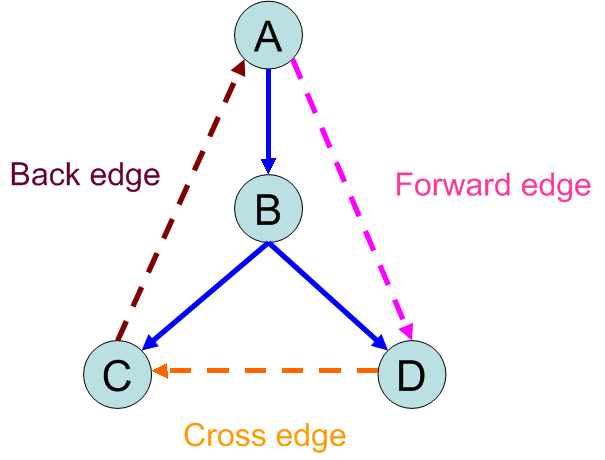
\includegraphics[width=0.50\textwidth]{figs/dfs-digraph.png}
	  \caption{DFS on directed graph.}
	\end{subfigure}%
	\begin{subfigure}{0.50\linewidth}
	  \centering
	  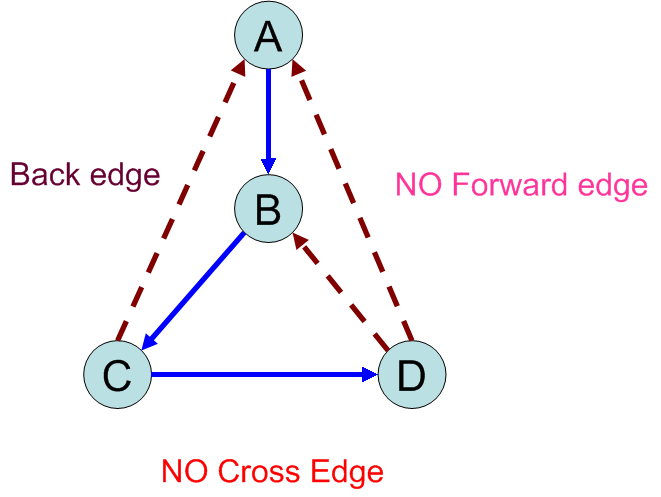
\includegraphics[width=0.50\textwidth]{figs/dfs-undirected.png}
	  \caption{DFS on undirected graph.}
	\end{subfigure}

	\begin{subfigure}{0.50\linewidth}
	  \centering
	  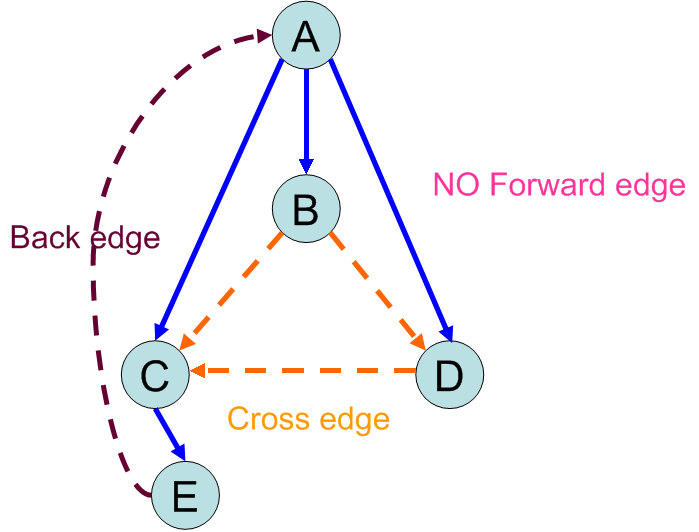
\includegraphics[width=0.50\textwidth]{figs/bfs-digraph.png}
	  \caption{BFS on directed graph.}
	\end{subfigure}%
	\begin{subfigure}{0.50\linewidth}
	  \centering
	  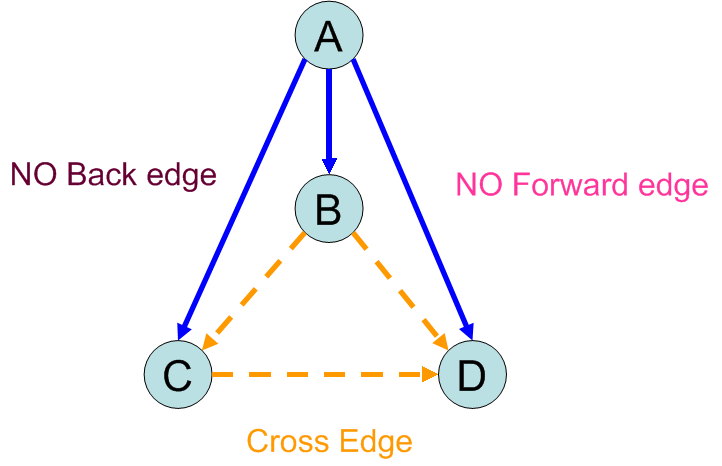
\includegraphics[width=0.60\textwidth]{figs/bfs-undirected.png}
	  \caption{BFS on undirected graph.}
	\end{subfigure}
  \end{figure}
\end{frame}
%%%%%%%%%%%%%%%%%%%%
\begin{frame}{Types of edges}
  \begin{exampleblock}{DFS tree and BFS tree coincide (Additional Problem)}
    \begin{itemize}
	  \item undirected connected graph $G = (V,E), v \in V$ 
	  \item DFS tree $T$ from $v$ $\equiv$ BFS tree $T'$ from $v$
      \item prove: $G = T$
    \end{itemize}
  \end{exampleblock}

  \pause
  \begin{center}
	$G_{\text{DFS}}$: tree + back \emph{vs.} $G_{\text{BFS}}$: tree + cross
  \end{center}

  \pause
  \begin{alertblock}{Question}
	\begin{itemize}
	  \item DFS\&BFS from different $v's$?
	  \item What if $G$ is a digraph?
	\end{itemize}
  \end{alertblock}
\end{frame}
%%%%%%%%%%%%%%%%%%%%
\begin{frame}{Lifttime of vertices in DFS}
  \fignocaption{width = 0.40\textwidth}{figs/active-interval.png}
\end{frame}
%%%%%%%%%%%%%%%%%%%%
\begin{frame}{Lifttime of vertices in DFS}
  \begin{theorem}[Disjoint or contained]
	\begin{gather*}
	  \forall u,v: \\
	  [_{u} \; ]_{u} \cap [_{v} \; ]_{v} = \emptyset \\
	  \bigvee \\
	  ([_{u} \; ]_{u} \subsetneqq [_{v} \; ]_{v} \lor [_{v} \; ]_{v} \subsetneqq [_{u} \; ]_{u})
	\end{gather*}
  \end{theorem}

  \pause

  \begin{proof}
	\fignocaption{width = 0.30\textwidth}{figs/stack.png}
  \end{proof}
\end{frame}
%%%%%%%%%%%%%%%%%%%%
\begin{frame}{Ancestor/descendant relation}
  \begin{exampleblock}{Preprocessing for ancestor/descendant relation (Problem 5.23)}
    \begin{itemize}
      \item binary tree $T = (V, E)$
      \item $r \in V$
    \end{itemize}
  \end{exampleblock}

  \[
	v: \text{d}[v], \text{f}[v]
  \]

  \pause
  \begin{alertblock}{Question}
    $\forall v$: how many descendants?
  \end{alertblock}

  \pause
  \begin{alertblock}{Remark}
	General (rooted) tree?
  \end{alertblock}
\end{frame}
%%%%%%%%%%%%%%%%%%%%
\begin{frame}{Edge types and lifetime of vertices in DFS}
  \begin{exampleblock}{Edge types and lifetime of vertices in DFS (Problem 5.2)}
    $\forall u \to v$:
    \begin{itemize}
      \item tree/forward edge: $[_{u}\; [_{v}\; ]_{v}\; ]_{u}$
      \item back edge: $[_{v}\; [_{u}\; ]_{u}\; ]_{v}$
      \item cross edge: $[_{v}\; ]_{v}\; [_{u}\; ]_{u}$
    \end{itemize}
  \end{exampleblock}

  \pause

  \begin{alertblock}{Remark}
    \begin{itemize}
      \item $\text{f}[v] < \text{d}[u]$: cross edge
      \item $\text{f}[u] < \text{f}[v]$: back edge
		\pause
		\[
		  u \to v \iff \text{f}[v] < \text{f}[u]
		\]
    \end{itemize}
  \end{alertblock}
\end{frame}
%%%%%%%%%%%%%%%%%%%%
\begin{frame}{Height and diameter of tree}
  \begin{exampleblock}{Height and diameter of tree (Problem 5.21)}
	Binary tree $T = (V, E)$ with $|V| = n$:
	\begin{itemize}
	  \item height ($O(n)$)
	  \item diameter ($O(n)$)
	\end{itemize}
  \end{exampleblock}

  \pause
  \vspace{0.30cm}
  \centerline{throught root or not?}

  \pause
  \vspace{0.50cm}
  \begin{alertblock}{Question}
	Diameter of a tree \emph{without} a designated root?
  \end{alertblock}
\end{frame}
%%%%%%%%%%%%%%%%%%%%
\begin{frame}{Perfect subtree}
  \begin{exampleblock}{Perfect subtree (Problem 5.22)}
	\begin{itemize}
	  \item binary tree $T = (V, E)$
	  \item root $r \in V$
	  \item goal: find all perfect subtrees
	\end{itemize}
  \end{exampleblock}
\end{frame}
%%%%%%%%%%%%%%%%%%%%
\begin{frame}{Counting shortest paths}
  \begin{exampleblock}{Counting shortest paths (Problem 5.26)}
	Counting \# of shortest paths in (un)directed graphs using BFS.
  \end{exampleblock}

  \pause
  \vspace{0.50cm}
  \centerline{Maybe in the next class$\dots$}
\end{frame}
%%%%%%%%%%%%%%%%%%%%
